\documentclass[sigplan,screen]{acmart}

%%
%% \BibTeX command to typeset BibTeX logo in the docs
\AtBeginDocument{%
  \providecommand\BibTeX{{%
    \normalfont B\kern-0.5em{\scshape i\kern-0.25em b}\kern-0.8em\TeX}}}

%% Rights management information.  This information is sent to you % when you
%complete the rights form.  These commands have SAMPLE % values in them; it is
%your responsibility as an author to replace % the commands and values with
%those provided to you when you % complete the rights form.
\setcopyright{acmcopyright}
\copyrightyear{2018}
\acmYear{2018} \acmDOI{10.1145/1122445.1122456}

\begin{document}
\title{Agent Path Planning}
\author{Noah Gardner}
\authornote{All authors contributed equally to this research.}
\email{ngardn10@students.kennesaw.edu}
\orcid{0000-0001-5900-9841}
\affiliation{%
    \institution{College of Computing and Software Engineering }
    \streetaddress{1100 South Marietta}
    \city{Marietta}
    \state{Georgia}
    \country{USA}
    \postcode{30060}
}

\author{Alan Norkham}
\email{@students.kennesaw.edu}
\affiliation{%
    \institution{College of Computing and Software Engineering }
    \streetaddress{1100 South Marietta}
    \city{Marietta}
    \state{Georgia}
    \country{USA}
    \postcode{30060}
}

\author{Mikulas Chalupa}
\email{@students.kennesaw.edu}
\affiliation{%
    \institution{College of Computing and Software Engineering }
    \streetaddress{1100 South Marietta}
    \city{Marietta}
    \state{Georgia}
    \country{USA}
    \postcode{30060}
}
\renewcommand{\shortauthors}{Gardner et al.}

\begin{abstract}
    The problem of path planning is a difficult problem for mobile robots. A
    practical example can be seen in the robots commonly employed in warehouses:
    they must navigate to pick up goods and move them to certain locations.
    Therefore, the robot needs a method of moving from an initial location in
    the warehouse to a final location repeatedly. In this paper, we propose a
    technique that allows a robot to path plan in generalized environments, from
    different starting and goal locations. The method is based on a graph
    representation of the environment, and is capable of finding the shortest
    path between two points in the environment. In order to generalize
    appropriately, we show that a neural network is able to effectively choose
    the correct actions to take at each time step in the path planning problem.
\end{abstract}
\keywords{path finding, deep reinforcement learning, djikstra's algorithm}
\maketitle

\section{Introduction}
Autonomous vehicles and mobile robotics must be able to navigate in environments
that are not completely known in advance, due to the nature of environments to
have unknown obstacles, such as other mobile objects and unknown terrains.
Effective path planning is required in order to make the most of scarce
resources such as time and energy. Additionally, safety should be considered in
environments where the robot works alongside other mobile objects, especially
humans.

We consider three criteria for efficient path planning: the path planning should
always be able to find an optimal path in a static environment, it must be able
to generalize to dynamic environments, and finally, it must minimize complexity,
storage, and computation \cite{janet_essential_1995}.

\section{Background and Related Work}
The need for path planning is borne from the increasing automation of
navigation. The autonomous agent needs to be able to plan a path based on the
limited amount of information given. This problem is explored by Nair et al. who
use an LSTM to guide an agent through a simulated environment
\cite{nair_robotic_2020}.

Yuan et al. also explore the problem, but with a novel Gated Recurrent
Unit-Recurrent Neural Network, and a more complex simulated environment. It is
our aim to at least reproduce and improve on the nair et al. work, as well as
expand the environmental generation complexity \cite{yuan_novel_2019}.

\section{Methodology}
Our goal for this project will to be to demonstrate a learned agent that can
pathfind effectively from the starting location to the goal location. In order
to do so, we will apply Dijkstra's algorithm to a custom grid-world environment
to find the ground truth path. We will simulate the agent to get a series of
experience tuples, which consist of the agent's action, the environment state,
and the reward. Then, we will use the experience tuples with rewards to train a
reinforcement learning algorithm based on RNN or LSTM.

\section{Dataset}
Our dataset is a set of generated matrices, which consist of a 'grid-world'
environment. The environment contains randomly placed agent, goal, and
obstacles. Since the locations of every element is randomized, our neural
network will have many disparate samples to learn from. In the current state,
the obstacles completely obstruct movement, but obstacles that have variable
traversal cost while still allowing movement are also planned.

\begin{figure}
    \centering
    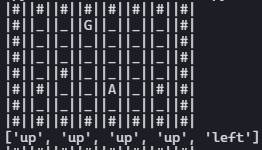
\includegraphics[width=0.45\textwidth]{assets/dataset/step0.png}
    \caption{Example starting state of the environment, where the agent is A,
        the goal is G, and the obstacles are $\#$. The agents path as a set of
        actions to reach the goal is also shown.}
    \label{fig:env_step0}
\end{figure}

\begin{figure}
    \centering
    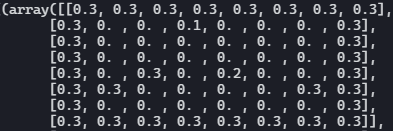
\includegraphics[width=0.45\textwidth]{assets/dataset/observation.png}
    \caption{Example observation of the starting state shown in fig.
        \ref{fig:env_step0}. Currently, the observation space is the same as the
        grid shape.}
    \label{fig:env_observation}
\end{figure}

\section{Model}
Typically in reinforcement learning, the model acts by itself in the
environment, and based on the rewards received, creates an optimal policy, a
series of actions to take to maximize it's rewards. In our case, we have access
to ground truth experience tuples from the environment, created from Dijkstra's
algorithm. Our method of training the model will be to use the ground truth
experience tuples in conjunction with the models own exploration of the
environment.

\section{Experimental Results}

\subsection{Experimental Setup and Metrics}
We would like to experiment with a novel parameter, $\alpha$ which will allow us
to train with our ground truth data. $\alpha$ is the percentage of experiences
which come from our 'perfect' agent's experiences. For example, if $\alpha$ is
0.5, then we will train our model with half of our ground truth data, and half
of the experiences collected by the agent. In the beginning of training, we will
set $\alpha$ to 1.0, and gradually decrease it to 0. Our experiments will
explore differences in different values of $\alpha$.

The performance of the model will be measured against Dijkstra's algorithm.
Since Dijkstra's will always find the path of least cost, the ratio between the
optimum and the path taken should be a good measure of efficiency. We can also
evaluate our model based on the number of steps taken to reach the goal or the
total reward received.

\subsection{Results}
No results at this time.

\section{Conclusion}
At this point in the project, we have finished the primary implementation of the
dataset: the environment in which the agent will act and the appropriate ground
truth experience tuples to use for training. However, we have an extra obstacle
we would like to implement, the sand pit, which the agent can move through, but
will have an extra cost of moving into. Ideally, the agent will learn to avoid
the sand pit where it can, but will move through it if it cannot. We also want
to implement a similar grid element which has a reduced cost of moving into it,
as if it were a road.

Currently, our environment shows the entire grid as the observation, but we will
implement a limited observation window around the agent for training LSTM. The
limited observation space will necessitate memory of prior states so the agent
will remember any obstacles. We are considering adding a goal direction to the
observation space as well.

We have run into some challenges in our implementation of the dataset so far,
but there are no major blockers at this point. We plan to continue moving
forward by finishing our extra grid elements, changing observation space, and
applying the model to run experiments.

\bibliographystyle{ACM-Reference-Format}
\bibliography{report}
\end{document}
